\documentclass[jkps,preprint,fleqn]{revtex4}
\usepackage{CJKutf8}
\usepackage[utf8]{inputenc}

\usepackage{graphicx}
\usepackage{amssymb}
\usepackage{amsmath}
\usepackage{bm}


\usepackage{pifont}
\newcommand{\cmark}{\ding{51}}
\newcommand{\xmark}{\ding{55}}
\usepackage{booktabs}
\usepackage{array}

\pdfoutput=1

\usepackage{float} \usepackage{graphicx}
\usepackage{epstopdf}
\usepackage{graphics}
\usepackage{caption}
\usepackage{subfigure}
\usepackage{epsfig}
\usepackage{color}
\usepackage{multirow,array}

\usepackage{tensor}

\usepackage{adjustbox}

\usepackage{tabularray}

\usepackage{hyperref}
\hypersetup{
	colorlinks=true,
	linkcolor=blue,
	filecolor=magneta,
	urlcolor=blue,
}

\usepackage{tikz}
\usetikzlibrary{3d}

\newcommand{\jn}[1]{{\color{blue} #1}}

\renewcommand{\topfraction}{0.8}
\renewcommand{\textfraction}{0.2}
\renewcommand{\floatpagefraction}{0.7}

\newcommand{\anal}{\text{anal}}
\newcommand{\eff}{\text{eff}}
\newcommand{\ine}{\text{inert}}
\newcommand{\cro}{\text{cr}}
\newcommand{\DE}{\text{DE}}
\newcommand{\m}{\text{m}}
\newcommand{\TA}{\text{A}}
\newcommand{\TB}{\text{B}}
\newcommand{\tf}{\tilde{f}}
\newcommand{\tF}{\tilde{F}}
\newcommand{\tR}{\tilde{R}}
\newcommand{\tg}{\tilde{g}}
\newcommand{\mg}{\mathcal{G}}
\newcommand{\mgg}{\mathcal{GG}}
\newcommand{\tmg}{\tilde{\mathcal{G}}}
\newcommand{\mL}{\mathcal{L}}
\newcommand{\mP}{\mathcal{P}}
\newcommand{\mA}{\mathcal{A}}
\newcommand{\tc}{\tilde{c}}
\newcommand{\ttc}{\tilde{\tilde{c}}}
\newcommand{\tG}{\tilde{G}}
\newcommand{\tT}{\tilde{T}}
\newcommand{\ta}{\tilde{a}}
\newcommand{\ps}{\text{ps}}
\newcommand{\tRR}{\tilde{R}}
\newcommand{\tSS}{\tilde{S}}
\newcommand{\tM}{\text{M}}
\newcommand{\TM}{\text{M}}
\newcommand{\TL}{\text{L}}
\newcommand{\TN}{\text{N}}
\newcommand{\SD}{\text{SD}}
\newcommand{\GR}{\text{GR}}
\newcommand{\EM}{\text{EM}}
\newcommand{\TBBN}{\text{BBN}}
\newcommand{\re}{\text{re}}
\newcommand{\rs}{\text{rs}}
\newcommand{\cm}{\text{cm}}
\newcommand{\Tp}{\text{p}}
\newcommand{\Teq}{\text{eq}}
\newcommand{\tgam}{\tilde{\gamma}}
\newcommand{\tlambda}{\tilde{\lambda}}
\newcommand{\tbeta}{\tilde{\beta}}
\newcommand{\tGam}{\tilde{\Gamma}}
\newcommand{\tkapp}{\tilde{\kappa}}
\newcommand{\trho}{\tilde{\rho}}
\newcommand{\tP}{\tilde{P}}
\newcommand{\tp}{\tilde{p}}
\newcommand{\Tn}{\text{n}}
\newcommand{\Tm}{\text{m}}
\newcommand{\Tr}{\text{r}}
\newcommand{\Tre}{\text{re}}
\newcommand{\Tc}{\text{c}}
\newcommand{\Tb}{\text{b}}
\newcommand{\Td}{\text{d}}
\newcommand{\Te}{\text{e}}
\newcommand{\Tw}{\text{w}}
\newcommand{\TW}{\text{W}}
\newcommand{\TT}{\text{T}}
\newcommand{\TtH}{\text{H}}
\newcommand{\TD}{\text{D}}
\newcommand{\Tde}{\text{de}}
\newcommand{\bbc}{\bar{c}}
\newcommand{\tih}{\tilde{h}}
\newcommand{\Tdrag}{\text{drag}}
\newcommand{\tnu}{\tilde{\nu}}
\newcommand{\tmu}{\tilde{\mu}}
\newcommand{\ttmu}{\tilde{\tilde{\mu}}}
\newcommand{\tepsilon}{\tilde{\epsilon}}
\newcommand{\ttepsilon}{\tilde{\tilde{\epsilon}}}
\newcommand{\Ch}{\text{Ch}}
\newcommand{\Tpc}{\text{pc}}
\newcommand{\TMpc}{\text{Mpc}}
\newcommand{\Temis}{\text{emis}}
\newcommand{\Tchirp}{\text{chirp}}
\newcommand{\Tgw}{\text{gw}}
\newcommand{\Ts}{\text{s}}
\newcommand{\Tret}{\text{ret}}
\newcommand{\Teff}{\text{eff}}
\newcommand{\Tobs}{\text{obs}}
\newcommand{\Tbias}{\text{bias}}
\newcommand{\Treq}{\text{req}}
\newcommand{\Tls}{\text{ls}}
\newcommand{\Tso}{\text{so}}
\newcommand{\YPBBN}{Y_{\text{P}}^{(\text{BBN})}}
\newcommand{\thbar}{\tilde{\hbar}}
\newcommand{\hTT}{\tilde{h}}

\newcommand{\defin}[1]{\textbf{\slshape #1}\index{#1}}

\newcommand{\of}[1]{\underset{\sim}{#1}}
\newcommand{\ovec}[1]{\overline{#1}}
\newcommand{\tvec}[1]{\overset{=}{#1}}

\newenvironment{remark}
{\begin{description} \item[\emph{备注:}]\em}
{\end{description}}

\newenvironment{example}[1][]
{\begin{description} 
\item[\emph{示例 #1 :}]\em}
{\end{description}}

\makeindex
\begin{document}
\begin{CJK*}{UTF8}{gbsn}
\setcounter{page}{0}

\title[]{重审宇宙学中的光速变化:弗里德曼-勒梅特-罗伯逊-沃尔克度规的启示}
\author{Seokcheon \surname{Lee}}
\email{skylee@skku.edu}
\affiliation{Department of Physics, Institute of Basic Science, Sungkyunkwan University, Suwon 16419, Korea}

\date[]{Received }

\begin{abstract}
在弗里德曼-勒梅特-罗伯逊-沃克度规中,光速可变(VSL)现象反映了超曲面上时钟速率的变化,这种变化由时移函数描述。该变化并非动力学场的演化,而是坐标选择的结果——由于外尔公设,宇宙时间与共动观测者的固有时保持一致。从包含$\tc$的作用量原理出发,我们推导出$\tc$本身不具有动力学特性,而是对尺度因子$a(t)$施加约束,表明其并非独立的自由度。这一认识将VSL概念重新阐释为广义相对论中规范自由度的体现,物理定律在光滑坐标变换下保持不变。此处"规范"指选择时间坐标的自由度(例如设定时移$N(t) \neq 1$),它决定了光速在宇宙学方程中的表现形式。将$\tc$理解为坐标依赖量,为解释宇宙学时间和观测矛盾(如哈勃张力)提供了新视角,而无需引入新的物理场。这种重新定义开辟了在自洽的相对论框架内解释宇宙膨胀的新理论路径。
\end{abstract}

\maketitle

\tableofcontents
\section{引言}
\label{sec:intro}

最小扩展变光速(meVSL)模型是在遵循宇宙学原理(CP)的弗里德曼-勒梅特-罗伯逊-沃克(FLRW)度规框架内建立的,该原理通过确保宇宙在大尺度上保持空间均匀性和各向同性来实现 \cite{Lee:2020zts,Lee:2023bjz,Lee:2024mal}。这一原理要求支配宇宙的物理定律不得引入优先方向或位置。维持这些对称性的关键要素是绝热性的守恒,因为宇宙介质中的任何净能流都将建立一个优先参考系,从而破坏各向同性 \cite{Lee:2022heb}。

在meVSL模型中,光速随宇宙时间的演化必须伴随其他基本物理常数的相应变化,以确保理论框架的内在一致性。特别是,普朗克常数必须与变化的光速协调演化,以保持解释绝热膨胀的量子力学和热力学基本关系 \cite{Lee:2022heb}。更广泛地说,必须诱导包括电磁相互作用和相对论动力学在内的其他物理量的宇宙学演化,以维持与所有局部验证物理定律(如狭义相对论和麦克斯韦方程组)的兼容性 \cite{Lee:2020zts,Lee:2023bjz,Lee:2024mal,Lee:2022heb}。

与传统VSL理论不同(后者通常需要显式机制来驱动$\tc$作为宇宙尺度因子$a(t)$的函数变化),meVSL模型不需要这种特设性规定。相反,它引入了宇宙时间膨胀(CTD)的广义条件,使得时间依赖的光速变化成为自然结果。在meVSL模型中,时移函数决定了超曲面间时钟速率的差异,反映了光速随时间的变化 \cite{Lee:2024zcu}。meVSL框架并非修改FLRW度规本身,而是允许$\tc$的变化从宇宙时间的底层结构中动态涌现,而无需强加特定的函数形式$\tc(a)$。

这一显著特征使meVSL区别于传统VSL模型——后者常假设或需要驱动光速演化的显式机制 \cite{Avelino:1999is,Belinchon:1999kq,Avelino:2000ph,Szydlowski:2002kz,Magueijo:2003gj,Shojaie:2004sq,Shojaie:2004xw,Balcerzak:2013kha,Balcerzak:2014rga,Franzmann:2017nsc,Hanimeli:2019wrt,Skara:2019usd,Bhattacharjee:2020fgl,Gupta:2020anq,Cuzinatto:2022mfe,Cuzinatto:2022vvy,Cuzinatto:2022dta,Bileska:2024odt,Coleman:1997xq,Albrecht:1998ir,Barrow:1998df,Barrow:1999is,Bassett:2000wj,Jacobson:2000xp,Magueijo:2000zt,Clayton:1998hv,Drummond:1999ut,Clayton:1999zs,Liberati:2000us,Clayton:2000xt,Drummond:2001rj,Amelino-Camelia:1996bln,Amelino-Camelia:1997ieq,Ellis:1999sd,Amelino-Camelia:2000bxx,Amelino-Camelia:2000cpa,Ellis:2000sf,Kowalski-Glikman:2001vvk,Bruno:2001mw,Magueijo:2001cr,Amelino-Camelia:2002uql,Magueijo:2002pg,Moffat:1992ud,Manida:1999rx,Barrow:1999st,Stepanov:1999ax,Magueijo:2000au,Moffat:2002nm,Kaelbermann:1998hu,Randall:1999ee,Randall:1999vf,Kiritsis:1999tx,Chung:1999xg,Alexander:1999cb,Ishihara:2000nf,Csaki:2000dm,Youm:2001sw,Youm:2001zk,Grojean:2001pv,Youm:2001zp,Drummond:1979pp,Novello:1988ma,Barton:1989dq,Scharnhorst:1990sr,Shore:1995fz,Colladay:1995qb,Coleman:1998ti,Bertolami:1999da,Shore:2000bs,Greenberg:2002uu,Teyssandier:2003qh,Shore:2003zc,Blasone:2003wf,Alexander:2001dr,Burgess:2002tb}。通过将基本常数的变化嵌入宇宙膨胀和时间膨胀的更广泛背景中,meVSL模型为探索膨胀宇宙中非固定光速的影响提供了更普适且自洽的路径。

本文结构如下:第2节简要概述现有VSL模型;第3节介绍meVSL模型背景下的FLRW度规,作为我们分析的基础;第4节讨论爱因斯坦-希尔伯特(EH)作用量,提供推导场方程的理论框架;第5节推导爱因斯坦场方程(EFEs),包括里奇张量、爱因斯坦张量、能量-动量张量及弗里德曼方程;第6节专述光速运动方程,探讨其在meVSL框架下的意义;最后第6节总结研究发现并讨论其广泛意义。
\section{现有变光速理论概述}
\begin{table}[htbp]
\centering
\caption{代表性VSL理论与meVSL框架的对比。}
\label{tab:VSLComparison}
\renewcommand{\arraystretch}{1.35}
\resizebox{\textwidth}{!}{
 \begin{tabular}{
    >{\raggedright\arraybackslash}p{3.2cm}
    >{\raggedright\arraybackslash}p{4.5cm}
    >{\centering\arraybackslash}p{1.2cm}
    >{\centering\arraybackslash}p{1.5cm}
    >{\centering\arraybackslash}p{1.5cm}
    >{\centering\arraybackslash}p{1.6cm}
    >{\raggedright\arraybackslash}p{2.8cm}
    >{\raggedright\arraybackslash}p{2.8cm}
}
\toprule
\hline
\textbf{Model} & \textbf{Variation Mechanism} & \textbf{Dyn} & \textbf{LI} & \textbf{New Fields} & \textbf{GR Covariance} & \textbf{Obs. Target} & \textbf{References} \\
\midrule
\hline
Hard Lorentz breaking & Preferred frame with $c(t)$ imposed explicitly & \xmark/\cmark & \xmark & \xmark/\cmark & \xmark & Conceptual variation & \cite{Coleman:1997xq,Albrecht:1998ir,Barrow:1998df,Barrow:1999is,Bassett:2000wj,Jacobson:2000xp,Magueijo:2000zt} \\
Bimetric VSL & $\hat{g}_{\mu\nu} = g_{\mu\nu} + B\partial_\mu\phi\partial_\nu\phi$ & \cmark & Partial & \cmark & Partial & Propagation delay & \cite{Clayton:1998hv,Drummond:1999ut,Clayton:1999zs,Liberati:2000us,Clayton:2000xt,Drummond:2001rj}  \\
Color-dependent VSL & $c(\nu)$ varies by frequency due to vacuum dispersion & \xmark & \xmark & \xmark & \xmark & High-energy astrophysics & \cite{Amelino-Camelia:1996bln,Amelino-Camelia:1997ieq,Ellis:1999sd,Amelino-Camelia:2000bxx,Amelino-Camelia:2000cpa,Ellis:2000sf,Kowalski-Glikman:2001vvk,Bruno:2001mw,Magueijo:2001cr,Amelino-Camelia:2002uql,Magueijo:2002pg} \\
Lorentz-invariant VSL & $c(x^\mu)$ as a scalar field in covariant framework & \cmark & \cmark & \cmark & \xmark & Model-dependent & \cite{Moffat:1992ud,Manida:1999rx,Barrow:1999st,Stepanov:1999ax,Magueijo:2000au,Moffat:2002nm} \\
String/M-theory & $c$ varies via compactification or brane motion & \cmark & \cmark & \cmark & Partial & Early-universe physics & \cite{Kaelbermann:1998hu,Randall:1999ee,Randall:1999vf,Kiritsis:1999tx,Chung:1999xg,Alexander:1999cb,Ishihara:2000nf,Csaki:2000dm,Youm:2001sw,Youm:2001zk,Grojean:2001pv,Youm:2001zp} \\
Field-theory VSL & $c = c(\phi)$ via scalar field $\phi$ & \cmark & Model-dep. & \cmark & \xmark & CMB, LSS, BBN &  \cite{Drummond:1979pp,Novello:1988ma,Barton:1989dq,Scharnhorst:1990sr,Shore:1995fz,Colladay:1995qb,Coleman:1998ti,Bertolami:1999da,Shore:2000bs,Greenberg:2002uu,Teyssandier:2003qh,Shore:2003zc,Blasone:2003wf} \\
Hybrid models & Combine metric and scalar field frameworks & \cmark & Model-dep. & \cmark & Model-dep. & Mixed datasets & \cite{Alexander:2001dr,Burgess:2002tb} \\
meVSL & Lapse function $N(t)$ chosen via coordinate freedom $\Rightarrow \tc(t)$ & \xmark & \cmark & \xmark & \cmark & CTD, $H_0$ tension & \cite{Lee:2020zts,Lee:2023ucu,Lee:2024kxa,Lee:2021ona,Lee:2023rqv,Lee:2024nya} \\
\bottomrule
\hline
\end{tabular}}
\end{table}
过去数十年间,学界提出了多种实现变光速(VSL)的理论框架,主要可分为以下几类:
\begin{itemize}
    \item \textbf{洛伦兹对称性的硬性破缺}:
    这类模型通过引入时空中的优先参考系或绝对结构,显式违反洛伦兹不变性 \cite{Coleman:1997xq,Albrecht:1998ir,Barrow:1998df,Barrow:1999is,Bassett:2000wj,Jacobson:2000xp,Magueijo:2000zt}。虽然能直接实现光速$c$的变化,但往往面临严重的理论困境,例如与相对性原理的冲突以及构建自洽量子场论的困难。
    
    \item \textbf{双度量变光速理论}:
    此类模型引入两个不同的度量:一个描述引力现象,另一个描述光子传播 \cite{Clayton:1998hv,Drummond:1999ut,Clayton:1999zs,Liberati:2000us,Clayton:2000xt,Drummond:2001rj}
\begin{align}
\hat{g}_{\mu\nu} = g_{\mu\nu} + B \partial_{\mu} \phi \partial_{\nu} \phi \label{bimetric} \,,
\end{align}
其中$g_{\mu\nu}$为引力子度量,$\hat{g}_{\mu\nu}$为物质度量,$\phi$为标量场。尽管保留了部分引力结构,双度量理论通常会引入额外的自由度,导致动力学复杂化,并引发稳定性和因果性问题。
    
    \item \textbf{色依赖的光速}:
    该框架允许光速随光子频率变化,从而建立真空色散关系 \cite{Amelino-Camelia:1996bln,Amelino-Camelia:1997ieq,Ellis:1999sd,Amelino-Camelia:2000bxx,Amelino-Camelia:2000cpa,Ellis:2000sf,Kowalski-Glikman:2001vvk,Bruno:2001mw,Magueijo:2001cr,Amelino-Camelia:2002uql,Magueijo:2002pg}。然而,此类色依赖变化受到天体物理观测(如伽马射线暴与引力波对应体)的严格限制,降低了其可行性。
    
    \item \textbf{洛伦兹不变的变光速理论}:
\end{itemize}
可以构建保持洛伦兹不变性本质的可变光速(VSL)理论。一种由Moffat~\cite{Moffat:1992ud}提出的方法涉及局域洛伦兹对称性的自发破缺,其中洛伦兹标量场获得类时真空期望值,从而选定一个优先参考系并将$O(3,1)$对称性破缺至$O(3)$。在此框架下,光速经历相变至当前较小值,而自发破缺方向为时间箭头与热力学第二定律提供了物理解释。另一方法~\cite{Magueijo:2000zt}则定义了协变且局域洛伦兹不变的场论,通过标量场$\psi = \log(c/c_0)$实现光速变化。根据模型参数,这些理论既可等价于标量-张量理论,也能定义全新框架。此类模型中,宇宙常数$\Lambda$可随$c$变化而作为$\psi$的势函数,通常满足$\Lambda \propto (c/c_0)^n$标度关系\cite{Manida:1999rx,Barrow:1999st,Stepanov:1999ax,Magueijo:2000au,Moffat:2002nm}。

\begin{itemize}
  \item \textbf{弦论/M理论方案}:
    在弦论或M理论中,$c$的变化可自然源于额外维动力学或演化标量场(模场)\cite{Kaelbermann:1998hu,Randall:1999ee,Randall:1999vf,Kiritsis:1999tx,Chung:1999xg,Alexander:1999cb,Ishihara:2000nf,Csaki:2000dm,Youm:2001sw,Youm:2001zk,Grojean:2001pv,Youm:2001zp}。
    尽管这些场景具有理论吸引力,但其高度依赖于紧致化方案与稳定化机制的假设,其中许多仍属推测性质。
   \item \textbf{场论VSL预言}:
    此类方法将$c$视为由动力学标量场驱动的有效耦合量\cite{Drummond:1979pp,Novello:1988ma,Barton:1989dq,Scharnhorst:1990sr,Shore:1995fz,Colladay:1995qb,Coleman:1998ti,Bertolami:1999da,Shore:2000bs,Greenberg:2002uu,Teyssandier:2003qh,Shore:2003zc,Blasone:2003wf}。
    虽然更贴近标准场论技术,但要确保规范不变性并与标准模型兼容仍需复杂构造。
    \item \textbf{混合模型}:
    部分模型综合上述要素,例如采用双度规结构与动力学标量场的组合\cite{Alexander:2001dr,Burgess:2002tb}。
    这些混合方案试图平衡各类优势,但往往同时继承多类别的理论挑战。
\end{itemize}

上述各类模型均面临非平凡障碍,尤其在保持基本对称性与观测数据吻合方面。相较之下,meVSL模型通过时移函数引入$\tc$的变化,将$\tc$的改变诠释为坐标效应而非引入新的物理自由度。这使得meVSL能在每一时刻保持CP不变性与相对性原理,提供了比传统VSL模型更简洁且对称的理论框架。表~\ref{tab:VSLComparison}总结了前述VSL模型与meVSL模型的差异。其中\textbf{Dyn}表示光速是否作为场方程支配的动力学量,\textbf{LI}指洛伦兹不变性,\textbf{Obs. Target}则标识各模型主要针对的观测现象。
\section{Friedmann-Lemaître-Robertson-Walker 度规}
\label{sec:RWm}
\begin{figure}
	\begin{center}
	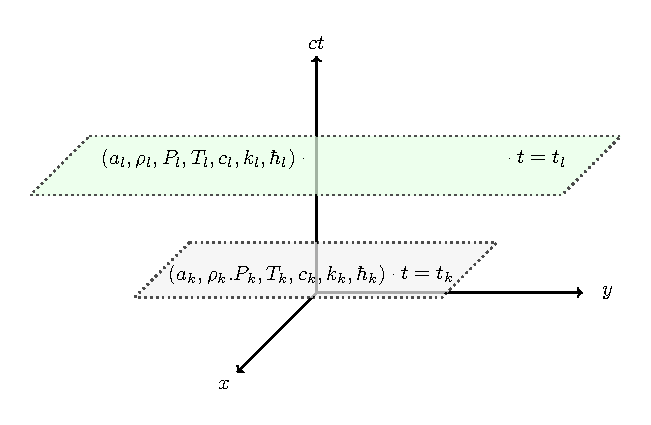
\includegraphics[width=0.9\textwidth]{Fig1.pdf}
	\caption{在 $t = t_k$ 时刻,物理量和常数的值(如 $a_k$、$\rho_k$、$P_k$、$T_k$、$\tc_k$、$k_{k}$ 和 $\hbar_k$)是固定的,且在 $t=t_k$ 超曲面上与空间位置无关。随着宇宙膨胀,这些量和常数会过渡为 $a_l$、$\rho_l$、$P_l$、$T_l$、$\tc_l$、$k_l$ 和 $\hbar_l$。宇宙学原理与外尔假设并未限制 $c_k$ 必须等于 $c_l$,其值由 CTD 关系决定。}
	\label{Fig1}
	\end{center}
\end{figure}
FLRW 度规建立在宇宙学原理(CP)之上,该原理假定宇宙在每一时刻都是均匀且各向同性的。数学上,这意味着生成空间各向同性和均匀性的基灵矢量(KVs)的李导数必须为零,从而确保度规在平移和旋转下保持不变 \cite{Lee:2024mal,Ryder09}。给定时刻 $t_l'$ 下各向同性且均匀空间的一般度规可表示为
\begin{equation}
g_{\mu\nu}^{(\text{CP})}(t_l') = \text{diag} \left( g_{00}(t_l') \,,  \frac{A(t_l')}{1-Kr^2} \,,  A(t_l') r^2 \,,  A(t_l') r^2 \sin^2 \theta \right) \,.
\end{equation}
对应的四维线元为
\begin{equation}
ds^2(t_l') = c_l^2 g_{00}(t_l') dt_l'^2 + A(t_l') \left[ \frac{dr^2}{1-Kr^2} + r^2 d \theta^2 + r^2 \sin^2 \theta d \phi^2 \right] \label{dstlp} \,,
\end{equation}
其中 $A(t_l') (= a^2(t_l'))$ 表示尺度因子的平方,而 \( g_{00}(t_l') \) 显式地由 \(- g_{00}(t_l') \equiv N^2(t_l') \) 给出,其中 \( N(t_l') \) 为时移函数 \cite{Lee:2024zcu,Ryder09}。通过采用外尔假设将式~\eqref{dstlp} 描述的度规推广到宇宙时 $t$,可将线元表示为
\begin{align}
ds^2 = - \tc(t)^2 dt^2 + a(t)^2 \left[ \frac{dr^2}{1-Kr^2} + r^2  \left( d \theta^2 + \sin^2 \theta d \phi^2 \right)  \right] \equiv - \tc(t)^2 dt^2 + a(t)^2 dl_{3\textrm{D}}^2 \label{dstgen} \,,
\end{align}
其中光速被视为时间的函数,这与标准 FLRW 度规中的传统角色不同(即 $N = 1$)。初看之下,这种表述可能显得非常规甚至错误。然而如图~\ref{Fig1} 所示,标准 FLRW 度规表明在 $t_l$ 或 $t_k$ 为常数的超曲面上,各类物理量——如尺度因子 $a_l = a(t_l)$、质量密度 $\rho_l$、压强 $P_l$、温度 $T_l$、光速 $\tc_l$、玻尔兹曼常数 $k_l$ 和普朗克常数 $\hbar_l$——在三维空间的所有空间位置保持恒定。但根据外尔假设,这些量可演化为宇宙时 $t$ 的函数,反映宇宙学红移效应,如图 \ref{Fig1} 所示。

传统宇宙学模型通常假设包括光速在内的物理常数不随时间变化。然而这种认为 $\tc_l$ 在整个宇宙时中恒等于 $\tc_k$ 的假设,并非推导 FLRW 度规的两个基本条件(即 CP 和外尔假设)的内在要求。实际上,光速不变性与共形时间导数(CTD)相关。需注意广义相对论(GR)并未规定任何要求光速保持不变的基本定律。当宇宙从 $t_k$ 演化至 $t_l$ 时,物理参数如 $a(t)$、$\rho(t)$、$P(t)$ 和 $T(t)$ 作为时间函数演化,其具体行为由求解爱因斯坦场方程(EFEs)和比安基恒等式(BI)决定,并考虑宇宙流体的状态方程(e.o.s)。

宇宙学中,可观测物理量通常不表示为宇宙时 $t$ 的函数,而是表示为宇宙学红移 $z$ 或等效尺度因子 $a(t) = 1/(1+z)$ 的函数。例如波长和温度等量会因宇宙膨胀而发生红移,这反映了时空的几何特性。从这个角度看,若带量纲的观测量自然随红移演化,那么考虑某些物理常数(特别是光速 $\tc$)也可能表示为红移函数就具有合理性。

FLRW 度规中时间坐标为 $x^0 = ct$,这表明若时移函数未固定,组合量 $\tc(t)$ 可被解释为如式~\eqref{NmeVSL} 所示的函数而非常数。这为理论提供了将标准宇宙学模型扩展至包含可变光速的可能性,且无需引入新的动力学场,而是通过 GR 内禀的规范自由度实现 \cite{Lee:2024zcu}。这种诠释构建了一个框架,其中传统上归因于常数 $\tc$ 的效应可能源于坐标选择,并为宇宙学现象提供新见解。

红移的推导源自光波传播的测地线方程,其中 $ds^2 = 0$ 条件成立,如式~\eqref{dstgen} 所示。在共动坐标系中,空间间隔 $dl_{3\textrm{D}}$ 随时间保持一致性 \cite{Lee:2024mal,Lee:2024zcu}。基于此框架,径向光传播表达式为
\begin{align}
d l_{3\textrm{D}} &= \frac{c(t_i) dt_i}{a(t_i)} \quad : \quad \frac{\tc_1 dt_1}{a_1} = \frac{\tc_2 dt_2}{a_2} \Rightarrow \begin{cases} \tc_1 = \tc_2 = c & \textrm{if} \quad \frac{dt_1}{a_1} = \frac{dt_2}{a_2} \qquad \textrm{SMC} \\
\tc_1 = \frac{f(a_2)}{f(a_1)} \frac{a_1}{a_2} \tc_2 & \textrm{if} \quad \frac{dt_1}{f(a_1)} = \frac{dt_2}{f(a_2)} \quad \textrm{VSL} \\ \tc_1 = \left( \frac{a_1}{a_2}\right)^{\frac{b}{4}} \tc_2 & \textrm{if} \quad \frac{dt_1}{a_1^{1-\frac{b}{4}}} = \frac{dt_2}{a_2^{1-\frac{b}{4}}} \quad \textrm{meVSL}  \end{cases} \,, \label{dl3D}
\end{align}
其中 $dt_i = 1/\nu(t_i)$ 表示 $t_i$ 时刻连续波峰间的时间间隔,对应于该时刻频率 $\nu_i$ 的倒数,而 $f(a_i)$ 是尺度因子 $a(t_i)$ 的任意函数。
在标准宇宙学模型(SMC)中,存在一个额外假设:光速保持恒定值$c$。这一假设源于广义相对论(GR)框架,其中$c$传统上被视为基本常数。因此,不同时间切片$t_1$和$t_2$下宇宙时间膨胀(CTD)与尺度因子倒数$a(t)$的关系可直接得出。然而,这种关系并非源自基本物理定律。相反,若如meVSL模型所提出的光速随时间变化,则传统的红移关系需要修正。

在膨胀宇宙中,从一个超曲面过渡到另一个超曲面会导致尺度因子增大,这自然会引起质量密度、温度等各种物理量的宇宙学红移。但仅凭宇宙学原理(CP)和韦尔假设,在FLRW度规框架内无法确证CTD关系。此类关系的验证需要依赖实验数据。旨在测量距离衰减时间的超新星(SNe)光变曲线和光谱的直接观测,为CTD测量提供了重要依据\cite{Leibundgut:1996qm,SupernovaSearchTeam:1997gem,Foley:2005qu,Blondin:2007ua,Blondin:2008mz,Lee:2023ucu,DES:2024vgg,Lee:2024kxa}。另一研究路径通过分析伽马射线暴(GRBs)峰间时间尺度的延长来探索CTD\cite{Norris:1993hda,Wijers:1994qf,Band:1994ee,Meszaros:1995gj,Lee:1996zu,Chang:2001fy,Crawford:2009be,Zhang:2013yna,Singh:2021jgr}。此外,遥远类星体(QSOs)的光变曲线也被用于检验潜在的CTD效应\cite{Hawkins:2001be,Dai:2012wp,Lewis:2023jab}。尽管存在这些努力,现有观测数据尚未明确证实CTD与SMC预测之间的关系。同时,FLRW模型缺乏确证CTD的明确机制。因此,只要结果与SMC预测相符,在这些观测中探索变光速(VSL)的可能性仍具价值。

鉴于FLRW模型理论上不包含CTD,若将该关系视为尺度因子的函数$f(a)$,则光速可表示为

\begin{align} \tc(t_1) = \frac{f(a_2)}{f(a_1)} \frac{a(t_1)}{a(t_2)} \tc(t_2) \label{cVSL}. \end{align}这凸显出:虽然广义相对论框架下VSL模型的普适性应用尚无法确证,但它作为FLRW度规描述的膨胀宇宙的自然结果而出现。meVSL模型是VSL的特例,由$f(a) = a^{1-b/4}$定义\cite{Lee:2020zts,Lee:2023bjz}。
\section{爱因斯坦-希尔伯特作用量}\label{sec:HEaction}

我们通过最小作用量原理,利用EH作用量推导爱因斯坦场方程(EFEs)。在变光速(VSL)模型中,光速是宇宙时间的函数。然而,若仅有光速为变量,帕拉蒂尼恒等式项会导致无法正确恢复爱因斯坦场方程。为解决此问题,必须允许引力常数($\tG$)也随宇宙时间变化,从而确保能从EH作用量获得正确的场方程形式\cite{Lee:2020zts}。这一条件保证了EH作用量中引力常数与光速的组合——即所谓的爱因斯坦引力常数$\tkapp \equiv 8 \pi \tG/\tc^4$——保持与宇宙时间无关。

VSL模型中的EH作用量可表述为
\begin{align} S &\equiv \int \Biggl[ \frac{1}{2 \tkapp} \left( R - 2 \Lambda \right) + \mathcal{L}_i \Biggr] \sqrt{-g} dt d^3x \label{SHmp} \,, \end{align}
其中$\mathcal{L}_i = \rho_i (1 + \omega_i) \tc^2$表示理想流体(即物质与辐射)的拉格朗日密度。如后文所示,在meVSL理论框架下,要确保从EH作用量恢复广义相对论的场方程,光速与引力常数必须同时发生宇宙学演化。

对作用量求逆度规变分并令其为零,可得
\begin{align} \delta S &= \int \left( \left[ \frac{\left( R - 2 \Lambda \right)}{2 \tkapp} \right] \delta \left( \sqrt{-g} \right)  + \frac{1}{2\tkapp} \sqrt{-g} \delta R \right) dt d^3 x + \int \delta \left( \sqrt{-g} \mathcal{L}{m} \right) dt d^3 x \nonumber \\ &= \int \frac{\sqrt{-g}}{2 \tkapp} \left[ R{\mu\nu} - \frac{1}{2} g_{\mu\nu} \left( R - 2 \Lambda \right) - \tkapp T_{\mu\nu} \right] \delta g^{\mu\nu} dtd^3 x \nonumber \\ &+ \int \frac{\sqrt{-g}}{2 \tkapp} \left[ \nabla_{\mu} \nabla_{\nu} - g_{\mu\nu} \Box \right] \delta g^{\mu\nu} dtd^3 x \label{deltaSHmp} \,. \end{align}
为保持爱因斯坦场方程,式~\eqref{deltaSHmp}中第二项(帕拉蒂尼恒等式项)必须为零。这意味着尽管$\tc$和$\tG$均随时间演化,$\tkapp$必须保持恒定:
\begin{align}
&\tkapp = \text{const} \quad \Rightarrow \quad \frac{\tG_0}{\tc_0^4} = \frac{\tG}{\tc^4} \quad \textrm{if} \quad \tc = \tc_0 f(a) \quad , \quad \tG = \tG_{0} f(a)^4 \label{tkappaconstmp} \,,
\end{align}
此处设$a_0 = 1$,$\tc_0$与$\tG_0$分别表示光速和引力常数的当前值。利用这些关系式,我们得到包含宇宙学常数的爱因斯坦场方程:
\begin{align} &R_{\mu\nu} - \frac{1}{2} g_{\mu\nu} R + \Lambda g_{\mu\nu} \equiv G_{\mu\nu} + \Lambda g_{\mu\nu}  = \frac{8 \pi \tG}{\tc^4} T_{\mu\nu} \label{tEFEmp} \,, \end{align}
该方程保持了广义相对论中场方程的标准协变形式。这表明变光速理论可被纳入广义相对论的协变框架,且不违背广义坐标变换下的基本对称性。
\section{爱因斯坦场方程} \label{sec:EFEs}

我们需要在变光速(VSL)理论框架下,利用FLRW度规和理想流体推导爱因斯坦场方程。通过这些方程,我们可以得到修正后的弗里德曼方程,进而将其与标准模型的相应方程进行对比分析差异。
\subsection{里奇张量与爱因斯坦张量}\label{subsec:RS}
我们现在利用FLRW度规推导VSL模型的EFEs\cite{Lee:2020zts,Lee:2025rpw}。由式~\eqref{dstgen}给出的FLRW度规的克里斯托费尔符号$\Gamma^{\mu}_{\,\,\nu\lambda}$为
\begin{align}
&\Gamma^{\mu}_{\,\,\nu\lambda} \equiv \frac{1}{2} g^{\mu\alpha} \left( g_{\alpha\nu,\lambda} + g_{\alpha\lambda,\nu} - g_{\nu\lambda,\alpha} \right) \label{Gamma}\,, \\ &\Gamma^{0}_{\,\,ij} = \frac{a\dot{a}}{\tc} \gamma{ij} \quad , \quad \Gamma^{i}_{\,\,0j} = \frac{1}{\tc}  \frac{\dot{a}}{a} \delta^i_j \quad , \quad \Gamma^{i}_{\,\,jk} = ^{s}\Gamma^{i}_{\,\,jk}  \label{Gammacomp} \,, \end{align}
其中$^{s}\Gamma^{i}_{\,\,jk}$表示空间度规$\gamma_{ij}$对应的克里斯托费尔符号。如式~\eqref{Gammacomp}所示,VSL模型中的克里斯托费尔符号形式与广义相对论中相同,唯一区别在于$\tc$是尺度因子的函数。

描述流形曲率的黎曼曲率张量由下式给出
\begin{align}
&\tensor{R}{^\alpha_\beta_\mu_\nu} = \tensor{\Gamma}{^\alpha_\beta_\nu_,_\mu} - \tensor{\Gamma}{^\alpha_\beta_\mu_,_\nu} + \tensor{\Gamma}{^\alpha_\lambda_\mu} \tensor{\Gamma}{^\lambda_\beta_\nu} - \tensor{\Gamma}{^\alpha_\lambda_\nu} \tensor{\Gamma}{^\lambda_\beta_\mu} \label{Rabmu} \,, \\ &\tensor{R}{^0_i_0_j} = \frac{\gamma_{ij}}{\tc^2} \left( a \ddot{a} - \dot{a}^2 \frac{d \ln \tc}{d \ln a} \right) \quad , \quad \tensor{R}{^i_0_0_j} = \frac{\delta^{i}{j}}{\tc^2} \left( \frac{\ddot{a}}{a} - \frac{\dot{a}^2}{a^2} \frac{d \ln \tc}{ d \ln a}  \right) \,, \label{R0i0j} \\ &\tensor{R}{^i_j_k_m} = \frac{\dot{a}^2}{\tc^2} \left( \delta^{i}{k} \gamma_{jm} - \delta^i_m \gamma_{jk} \right) + \tensor[^s]{R}{^i_j_k_m} \quad , \quad \tensor[^s]{R}{^i_j_k_m} = k \left( \delta^i_k \gamma_{jm} - \delta^i_m \gamma_{jk} \right) \,. \label{Rijkm} \end{align}
虽然VSL模型中的克里斯托费尔符号形式与广义相对论相同,但黎曼曲率张量存在差异。这种差异源于黎曼曲率张量是通过对克里斯托费尔符号求导得到的,而后者包含时变光速。这导致修正项的出现,例如$H^2 \frac{d \ln \tc}{d \ln a}$因子同时出现在$\tensor{R}{^0_i_0_j}$和$\tensor{R}{^i_0_0_j}$中。

测量沿测地线运动时空间形变的里奇曲率张量,可通过收缩式~\eqref{R0i0j}和\eqref{Rijkm}中的黎曼曲率张量获得
\begin{align}
R_{\mu\nu} &= \tensor{\Gamma}{^\lambda_\mu_\nu_,_\lambda} - \tensor{\Gamma}{^\lambda_\mu_\lambda_,_\nu} + \tensor{\Gamma}{^\lambda_\mu_\nu} \tensor{\Gamma}{^\sigma_\lambda_\sigma} - \tensor{\Gamma}{^\sigma_\mu_\lambda} \tensor{\Gamma}{^\lambda_\nu_\sigma} \label{Rmn} \,, \\ R_{00} &= -\frac{3}{\tc^2} \left( \frac{\ddot{a}}{a} - \frac{\dot{a}^2}{a^2} \frac{d \ln \tc}{ d \ln a}  \right) \quad , \quad R_{ij} = \frac{\gamma_{ij}}{\tc^2} a^2 \left( 2 \frac{\dot{a}^2}{a^2} + \frac{\ddot{a}}{a} + 2 k \frac{\tc^2}{a^2} - \frac{\dot{a}^2}{a^2} \frac{d \ln \tc}{ d \ln a}  \right) \label{Rij} \,. \end{align}
$\tc$的时变特性在$R_{00}$和$R_{ij}$中都引入了修正项。

最后,通过对里奇张量求迹可获得里奇标量
\begin{align} R &= \frac{6}{\tc^2} \left( \frac{\ddot{a}}{a} + \frac{\dot{a}^2}{a^2} + k \frac{\tc^2}{a^2} - \frac{\dot{a}^2}{a^2} \frac{d \ln \tc}{ d \ln a}  \right) =  \frac{6}{\tc^2} \left( \frac{\ddot{a}}{a} + \frac{\dot{a}^2}{a^2} + k \frac{\tc^2}{a^2} - \frac{\dot{a}}{a} \frac{\dot{\tc}}{\tc}  \right)  \label{Rmp} \,, \end{align}
其中光速时变效应在末项中表现明显。

爱因斯坦张量定义如下
\begin{align}
G_{\mu\nu} = R_{\mu\nu} - \frac{1}{2} g_{\mu\nu} R \label{Gmunu} \,.
\end{align}
利用先前推导的里奇张量~\eqref{Rij}和里奇标量~\eqref{Rmp},我们现在可以得到爱因斯坦张量的分量
\begin{align}
G_{00} = \frac{3}{\tc^2} \left[ \frac{\dot{a}^2}{a^2} + k \frac{\tc^2}{a^2} \right] \quad , \quad G_{ij} = -\frac{g_{ij}}{\tc^2} \left[ 2 \frac{\ddot{a}}{a} + \frac{\dot{a}^2}{a^2} + k \frac{\tc^2}{a^2} - 2 \frac{\dot{a}^2}{a^2} \frac{d \ln \tc}{d \ln a} \right] \,. \label{G00Gij}
\end{align}
这两个分量的BI关系可通过式~\eqref{G00Gij}简单证明
\begin{align}
\nabla_{\mu} G^{\mu \nu} = 0 \label{nablaGmunu} \,.
\end{align}
\subsection{能量动量张量}\label{subsec:Tmunu}

为了求解方程\eqref{tEFEmp}给出的爱因斯坦场方程,必须将应力-能量张量(SET)与方程~\eqref{Rij}和\eqref{Rmp}中的几何量相结合。对于作为时空曲率源的热力学平衡态理想流体,其SET具有对称形式
\begin{align} T_{\mu\nu} = \left( \rho + \frac{P}{\tc^2} \right) U_{\mu} U_{\nu} + P g_{\mu\nu} \label{Tmunump} \,, \end{align}
其中$\rho$表示质量密度,$P$代表流体静压,$U^{\mu} = (\tc\,,\vec{0})$为四维速度。爱因斯坦张量$G_{\mu\nu}$与度规张量$g_{\mu\nu}$满足一个关键几何恒等式——比安基恒等式\eqref{nablaGmunu}及度规相容性条件(即$\nabla_{\mu} g^{\mu\nu} = 0$)。鉴于爱因斯坦引力常数$\kappa$为常量,比安基恒等式直接导出能量动量局域守恒律
\begin{align} &\nabla_{\mu} \tensor{T}{^\mu^\nu} = 0 \quad \Rightarrow \quad \frac{\partial \rho_i}{\partial t} + 3 H \left( \rho_i + \frac{P_i}{\tc^2} \right) + 2 \rho_i H \frac{d \ln \tc}{d \ln a} = 0 \nonumber \\ &\Rightarrow d \ln \left( \rho_i \tc^2 \right) + 3 \left( 1 + \omega_i \right) d \ln a = 0 \label{BI1mp} \,, \end{align}
此处$\omega_i$为状态方程参数,定义为$\omega_i = (P_i/\tc^2)/\rho_i$。

求解方程~\eqref{BI1mp}可得能量密度的表达式
\begin{align} &\rho_i \tc^{2} = \rho_{i0} \tc_0^2 a^{-3 (1 + \omega_i)} \label{rhomp} \,,\end{align}
其中$i$代表对应于辐射或物质的理想流体组分。
\subsection{弗里德曼方程}\label{subsec:FE}

将式~\eqref{Rij}、~\eqref{Rmp}、~\eqref{Tmunump} 和 ~\eqref{rhomp} 代入式~\eqref{tEFEmp} 后,VSL 模型的爱因斯坦场方程可表示为
\begin{align}
 &\frac{\dot{a}^2}{a^2} + k \frac{\tc^2}{a^2}  -\frac{ \Lambda \tc^2}{3} = \frac{8 \pi \tG}{3} \sum_i \rho_i \label{tG00mp} \,, \\
 &\frac{\dot{a}^2}{a^2} + 2 \frac{\ddot{a}}{a} +  k \frac{\tc^2}{a^2} - \Lambda \tc^2 - 2 \frac{\dot{a}^2}{a^2} \frac{d \ln \tc}{d \ln a} = -\frac{8 \pi \tG}{\tc^2} \sum_{i} P_i  \label{tG11mp} \,.
 \end{align}
这些是由 VSL 效应修正后的弗里德曼方程。根据式~\eqref{tG00mp} 和 \eqref{tG11mp},宇宙膨胀加速度的控制方程为
\begin{align}
 \frac{\ddot{a}}{a} = -\frac{4\pi \tG}{3} \sum_i \left( 1 + 3 \omega_i \right) \rho_i  + \frac{\Lambda \tc^2}{3} + \frac{\dot{a}^2}{a^2} \frac{d \ln \tc}{d \ln a} \label{t3G11mG00mp} \,.
 \end{align}
通过式~\eqref{tkappaconstmp} 和 \eqref{rhomp} 重写哈勃参数 $H$ 和加速度 $\ddot{a}/a$,可得
\begin{align}
 H^2 &= \left[ \frac{8 \pi \tG_0}{3} \sum_{i} \rho_{0i} a^{-3(1+\omega_i)} + \frac{ \Lambda \tc_0^2}{3} - k \frac{\tc_0^2}{a^2} \right] \frac{\tc^2}{\tc_0^2} \equiv H^{(\GR)2} \frac{\tc^2}{\tc_0^2} \label{H2me} \,, \\
 \frac{\ddot{a}}{a} &= \left[ -\frac{4\pi \tG_0}{3} \sum_i \left( 1 + 3 \omega_i \right) \rho_{0i} a^{-3(1+\omega_i)} + \frac{\Lambda \tc_0^2}{3} \right] \frac{\tc^2}{\tc_0^2} + H^2 \frac{d \ln \tc}{d \ln a} \nonumber \\
 &= \left[ \left( \frac{\ddot{a}}{a} \right)^{(\GR)} +  H^{(\GR)2} \frac{d \ln \tc}{d \ln a}  \right] \frac{\tc^2}{\tc_0^2} \label{ddotaoa} \,.
 \end{align}
这些方程描述了 VSL 框架下 FLRW 宇宙的背景演化。VSL 模型中的哈勃膨胀率 $H$ 相较于广义相对论中的对应量 $H^{(\GR)}$ 多了一个附加因子 $\tc^2/\tc_0^2$。值得注意的是,虽然当前时刻的哈勃参数在广义相对论与 VSL 模型中保持一致,但其历史演化过程存在差异。过去更高的(或更低的)光速会导致按比例更大(或更小)的 $H$ 值。这种独特的标度行为可能为解决哈勃张力提供新思路。

此外,meVSL 模型中宇宙膨胀加速度的修正主要来自两个关键效应:第一项源于 $\tc$ 变化的额外项 $d \ln \tc/d \ln a$;第二项对应整体标度因子 $\tc^2/\tc_0^2$,导致膨胀率的相应修正。这些偏差凸显了 meVSL 框架引入的宇宙演化本质差异。

尽管如式~\eqref{H2me} 所示,meVSL 模型给出的哈勃参数 $H(a)$ 与标准宇宙学模型 $H^{\textsuperscript{\tiny (\GR)}}(a)$ 不同,但由此得到的哈勃半径
\begin{equation}
    \frac{\tilde{c}(a)}{H(a)}  = \frac{\tc_0}{H^{\textsuperscript{\tiny (\GR)}}(a)} = \frac{\tilde{c}_0}{H_0} \frac{1}{\sqrt{\sum_i \Omega_{0i} a^{-3(1+w_i)} + \Omega_\Lambda + \Omega_k a^{-2}}},
\end{equation}
仍与标准模型保持一致。这是因为 $\tilde{c}(a)$ 的构建旨在保持时空因果结构不变。因此,只要红移定义相同,诸如光度距离和角直径距离等可观测量——作为红移函数对哈勃半径的积分——在 meVSL 框架下将与标准模型给出相同结果~\cite{Lee:2020zts}。这意味着局部测量的 $H_0$ 值(如 SH0ES 结果)与距离指标推算值之间的差异可能在 meVSL 方法中得到调和~\cite{Lee:2024nya}。然而,若 $\tilde{c}$ 的变化影响其他物理常数(如精细结构常数、普朗克常数或钱德拉塞卡质量),则可能产生额外的观测效应~\cite{Lee:2020zts,Lee:2021xwh},导致超新星距离模数或最后散射面位置出现可检测的差异。关于这些影响的详细分析,请参阅文献~\cite{Lee:2020zts}。
\section{光速运动方程}
\label{sec:sol}

式~\eqref{SHmp}给出的作用量明确包含了式~\eqref{Rmp}中的里奇标量及理想流体项,其形式可表示为
\begin{align}
S &\equiv \int \Biggl[ \frac{1}{2 \tkapp} \left( \frac{6}{\tc^2} \left( \frac{\ddot{a}}{a} + \frac{\dot{a}^2}{a^2} + k \frac{\tc^2}{a^2} - \frac{\dot{a}}{a} \frac{\dot{\tc}}{ \tc} \right)  - 2 \Lambda \right) + \sum_{i=r\,,m} \rho_i (1 + \omega_i ) \tc^2 \Biggr] \sqrt{-g} dt d^3x \label{SHmppf} \,.
\end{align}
在方程~\eqref{SHmppf}中,理想流体的拉格朗日量看似显式依赖于$\tc$。然而根据理想流体的BI方程~\eqref{rhomp},可以证明该项与$\tc$无关
\begin{align}
 \rho_i (1 + \omega_i ) \tc^2 =  \rho_{i0} (1 + \omega_i ) \tc_{0}^2 a^{-3(1 + \omega_i )}  \label{rhoi} \,.
\end{align}
此外,由于爱因斯坦引力常数$\tkapp$具有时间无关性(如方程~\eqref{tkappaconstmp}所示),方程~\eqref{SHmppf}可改写为仅含$\tc$与$\dot{\tc}$项的形式
\begin{align}
S &= \int \Biggl[ \frac{\tc_0^4}{16 \pi \tG_0} \left( \frac{6}{\tc^2} \left( \frac{\ddot{a}}{a} + \frac{\dot{a}^2}{a^2} + k \frac{\tc^2}{a^2} - \frac{\dot{a}}{a} \frac{\dot{\tc}}{ \tc} \right)  - 2 \Lambda \right)  \Biggr] \sqrt{-g} dt d^3x \equiv \int \frac{1}{2 \tkapp_0} R \sqrt{-g} dt d^3x \label{SHmppf2} \,.
\end{align}
由式~\eqref{SHmppf2}可导出关于$c$的欧拉-拉格朗日方程
\begin{align}
& \frac{d}{dt} \frac{\partial R}{\partial \dot{\tc}} - \frac{\partial R}{\partial \tc} = 0 \quad \Rightarrow \quad \frac{\ddot{a}}{a} + 3 \frac{\dot{a}^2}{a^2} = 0 \quad \Rightarrow \quad a(t) = (c_1 + c_2 t)^{1/4} \label{eomtc} \,.
\end{align}
通常欧拉-拉格朗日方程应决定给定变量的动力学行为。但在求解$\tc$的方程时,我们发现其并未给出$\tc$本身的动力学方程,而是导致对$a(t)$的约束条件。这意味着$\tc$并非独立的动力学自由度,而是作为强制施加于$a(t)$特定约束的参数。

这表明$a(t)$与$\tc$的独立变量关系仅在特定条件下成立。这种关联性揭示了$\tc$与$a$之间的强依赖性,暗示$\tc$可能并非完全独立的物理量。$\tc$的变化与我们定义时间的方式密切相关。如果$\tc$始终仅作为$a(t)$的函数被确定,很可能是因为我们所采用的时间定义已被固定为特定形式。因此,若能重新定义时间,或许可将$\tc$视为独立变量。反之,若$\tc$在任何时间变量选择下都依赖于$a(t)$,则$\tc$本质上更可能是个因变量。

\begin{figure}
	\begin{center}
	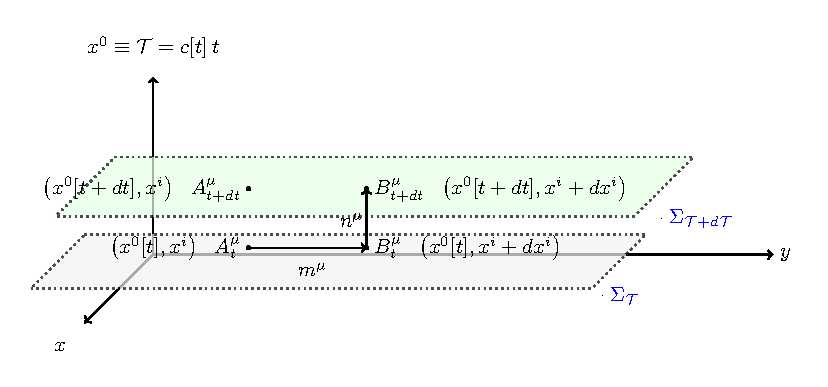
\includegraphics[width=0.9\textwidth]{Fig2.pdf}
	\caption{该图展示了RW度规框架下时空的叶状结构。超曲面$\Sigma$表示时间坐标$\mathcal{T}$的常数值,对应于不同的时间时刻。流逝函数控制着这些超曲面之间的间距,确保法向量$\bar{n} = n^{\mu} e_{\mu}$始终与它们保持正交。}
	\label{Fig2}
	\end{center}
\end{figure}

在meVSL模型中,时移函数描述了$\tc$的变异。我们可将时移函数定义为$N \equiv \tc/c$
\begin{align}
x^{0}(t+dt) - x^{0}(t) &=  \left( c[t+dt] \right) \left( t+dt \right) - c(t) t \overset{\mathcal{O}(1)}{\approx} c[t] dt + dc[t] t \nonumber \\
	&= \left( 1 + \frac{d \ln c}{d \ln t} \right) c[t] dt \equiv \tilde{c}[t] dt \equiv N[t] c[t] dt \label{NmeVSL} \,.
\end{align}
通过时移函数表征$\tc$变化的能力意味着,$\tc$的改变并非纯粹的物理动力学过程,而是取决于所选时间变量的定义。因此,$\tc$更可能是由坐标选择(时移函数)决定的量,而非独立变量。换言之,有必要重新考量$\tc$应被视为独立动力学自由度,还是应通过时移函数解释为坐标效应。

在meVSL模型中,时移函数表征了各超曲面上的时间流逝。若不存在确定时移函数的机制,则关于$\tc$的欧拉-拉格朗日方程并不描述动力学演化,而仅给出约束方程。$\tc$可通过时移函数表达的事实表明,它并非独立的动力学自由度,而是由坐标选择决定的量。因此,在缺乏额外机制固定时移函数的情况下,$\tc$不能被视作真正独立的变量。

时移函数$N(t)$决定了固有时间相对于坐标时间的流逝速率,在时空叶状结构中反映了时间切片的任意性,编码了空间超曲面间的时间推进方式。物理上,它设定了共动观测者经历的时间钟率,意味着变化的时移函数对应非平庸的时间规范。在meVSL框架下,这使我们能将有效光速$\tc(t)$的时间依赖性解释为时移函数选择的结果,而非源自独立场动力学。这种解释保持了广义相对论的广义协变性,并将$\tc$的变异重新定义为坐标效应而非新物理学的征兆。
\section{结论与总结}\label{sec:Conc}
本工作中,我们研究了罗伯逊-沃克度规下光速可变性的物理意义。研究表明,$\tc$的变化在此语境下并不必然意味着光速发生了根本性的物理改变,而是反映了与宇宙时间选择相关的坐标效应。

关键发现在于:RW度规中的宇宙时间与共动观测者的固有时相同,这一性质由外尔公设保证。在此设定下,可变光速对应的是超曲面间钟速的变化,而非内在的物理演化。这一解释通过从包含$\tc$的作用量推导欧拉-拉格朗日方程得到强化——所得方程并不描述$c$自身的动力学,而是对尺度因子$a(t)$的演化施加约束。这表明$\tc$并非独立自由度,而是依赖于宇宙时间流逝函数。

对VSL的这种重新诠释挑战了宇宙学中的传统假设。许多VSL模型认为$\tc$的变化代表时空物理的根本修改,常引入额外假设或机制来证明这种变化。然而我们的分析表明,这些变化可被理解为坐标选择的结果,而非需要新物理。在此视角下,$\tc$的表观演化反映的是宇宙时间结构的参数化方式,而非光传播的实际改变。

综上所述,我们的研究结果表明:可变光速是宇宙时间的坐标依赖特征,而非物理定律的根本修改。这一认识为VSL模型及其宇宙学意义(特别是宇宙膨胀和观测张力方面)提供了新视角。需要进一步研究该框架能否为现代宇宙学关键问题提供更一致、更自然的解决方案。

该方法也可能为当前观测张力(如哈勃张力或Ia型超新星时间膨胀异常)提供新解释,且无需引入新的动力学自由度。需进一步探究该框架能否一致重现宇宙学可观测量(如光度距离-红移关系),以及能否为标准宇宙学模型提供可行替代方案。作为规范选择,我们可以任意设定可变光速的形式为$\tc = \tc_0 a^{b/4}$。通过将该参数化与Ia型超新星时间膨胀测量等宇宙学观测对比,可检验$b$值是否偏离零。若观测数据倾向于$b \neq 0$,则表明常用规范选择$b = 0$(对应标准宇宙学模型)可能未能准确描述宇宙的时间结构;反之若$b = 0$仍被支持,则强化标准规范与观测的一致性。

\acknowledgments{本研究由韩国国家研究基金会(NRF)资助,资金来源为教育部(资助编号NRF-RS202300243411)。}
\begin{thebibliography}{999}
\bibitem{Lee:2020zts}
S.~Lee,
JCAP \textbf{08}, 054 (2021)
doi:10.1088/1475-7516/2021/08/054
[arXiv:2011.09274 [astro-ph.CO]].
\bibitem{Lee:2023bjz}
S.~Lee,
Found. Phys. \textbf{53}, 40 (2023)
doi:10.1007/s10701-023-00682-1
[arXiv:2303.13772 [physics.gen-ph]].
\bibitem{Lee:2024mal}
S.~Lee,
Particles \textbf{7}, no.2, 309-326 (2024)
doi:10.3390/particles7020019
[arXiv:2406.02556 [physics.gen-ph]].
\bibitem{Lee:2022heb}
S.~Lee,
Phys. Dark Univ. \textbf{42}, 101286 (2023)
doi:10.1016/j.dark.2023.101286
[arXiv:2212.03728 [astro-ph.CO]].
\bibitem{Lee:2024zcu}
S.~Lee,
Class. Quant. Grav. \textbf{42}, no.2, 025026 (2025)
doi:10.1088/1361-6382/ada2d5
[arXiv:2412.19049 [gr-qc]].
\bibitem{Avelino:1999is}
P.~P.~Avelino and C.~J.~A.~P.~Martins,
Phys. Lett. B \textbf{459} (1999), 468-472
doi:10.1016/S0370-2693(99)00694-2
[arXiv:astro-ph/9906117 [astro-ph]].
\bibitem{Belinchon:1999kq}
J.~A.~Belinchon,
Int. J. Theor. Phys. \textbf{39}, 1669-1686 (2000)
doi:10.1023/A:1003644614145
[arXiv:gr-qc/9907003 [gr-qc]].
\bibitem{Avelino:2000ph}
P.~P.~Avelino, C.~J.~A.~P.~Martins and G.~Rocha,
Phys. Lett. B \textbf{483} (2000), 210
doi:10.1016/S0370-2693(00)00567-0
[arXiv:astro-ph/0001292 [astro-ph]].
\bibitem{Szydlowski:2002kz}
M.~Szydlowski and A.~Krawiec,
Phys. Rev. D \textbf{68}, 063511 (2003)
doi:10.1103/PhysRevD.68.063511
[arXiv:gr-qc/0212068 [gr-qc]].
\bibitem{Magueijo:2003gj}
J.~Magueijo,
Rept. Prog. Phys. \textbf{66}, 2025 (2003)
doi:10.1088/0034-4885/66/11/R04
[arXiv:astro-ph/0305457 [astro-ph]].
\bibitem{Shojaie:2004sq}
H.~Shojaie and M.~Farhoudi,
Can. J. Phys. \textbf{85}, 1395-1408 (2007)
doi:10.1139/P07-132
[arXiv:gr-qc/0406027 [gr-qc]].
\bibitem{Shojaie:2004xw}
H.~Shojaie and M.~Farhoudi,
Can. J. Phys. \textbf{84}, 933-944 (2006)
doi:10.1139/P06-070
[arXiv:gr-qc/0407096 [gr-qc]].
\bibitem{Balcerzak:2013kha}
A.~Balcerzak and M.~P.~Dabrowski,
Phys. Lett. B \textbf{728}, 15-18 (2014)
doi:10.1016/j.physletb.2013.11.029
[arXiv:1310.7231 [astro-ph.CO]].
\bibitem{Balcerzak:2014rga}
A.~Balcerzak and M.~P.~Dabrowski,
JCAP \textbf{06}, 035 (2014)
doi:10.1088/1475-7516/2014/06/035
[arXiv:1406.0150 [astro-ph.CO]].
\bibitem{Franzmann:2017nsc}
G.~Franzmann,
[arXiv:1704.07368 [gr-qc]].
\bibitem{Hanimeli:2019wrt}
E.~T.~Hanımeli, B.~Lamine, A.~Blanchard and I.~Tutusaus,
Phys. Rev. D \textbf{101}, no.6, 063513 (2020)
doi:10.1103/PhysRevD.101.063513
[arXiv:1910.08325 [astro-ph.CO]].
\bibitem{Skara:2019usd}
F.~Skara and L.~Perivolaropoulos,
Phys. Rev. D \textbf{101}, no.6, 063521 (2020)
doi:10.1103/PhysRevD.101.063521
[arXiv:1911.10609 [astro-ph.CO]].
\bibitem{Bhattacharjee:2020fgl}
S.~Bhattacharjee and P.~K.~Sahoo,
Eur. Phys. J. Plus \textbf{135}, no.1, 86 (2020)
doi:10.1140/epjp/s13360-020-00116-1
[arXiv:2001.06569 [gr-qc]].
\bibitem{Gupta:2020anq}
R.~P.~Gupta,
doi:10.1093/mnras/staa2472
[arXiv:2009.08878 [astro-ph.CO]].
\bibitem{Cuzinatto:2022dta}
R.~R.~Cuzinatto, R.~P.~Gupta, R.~F.~L.~Holanda, J.~F.~Jesus and S.~H.~Pereira,
Mon. Not. Roy. Astron. Soc. \textbf{515}, no.4, 5981-5992 (2022)
doi:10.1093/mnras/stac2039
[arXiv:2204.10764 [gr-qc]].
\bibitem{Cuzinatto:2022mfe}
R.~R.~Cuzinatto, R.~F.~L.~Holanda and S.~H.~Pereira,
Mon. Not. Roy. Astron. Soc. \textbf{519}, 633-640 (2023)
doi:10.1093/mnras/stac3267
[arXiv:2202.01371 [gr-qc]].
\bibitem{Cuzinatto:2022vvy}
R.~R.~Cuzinatto, R.~P.~Gupta and P.~J.~Pompeia,
Symmetry \textbf{15}, no.3, 709 (2023)
doi:10.3390/sym15030709
[arXiv:2204.00119 [gr-qc]].
\bibitem{Bileska:2024odt}
M.~Bileska,
Class. Quant. Grav. \textbf{41}, no.18, 183001 (2024)
doi:10.1088/1361-6382/ad68f0
\bibitem{Coleman:1997xq}
S.~R.~Coleman and S.~L.~Glashow,
Phys. Lett. B \textbf{405}, 249-252 (1997)
doi:10.1016/S0370-2693(97)00638-2
[arXiv:hep-ph/9703240 [hep-ph]].
\bibitem{Albrecht:1998ir}
A.~Albrecht and J.~Magueijo,
Phys. Rev. D \textbf{59}, 043516 (1999)
doi:10.1103/PhysRevD.59.043516
[arXiv:astro-ph/9811018 [astro-ph]].
\bibitem{Barrow:1998df}
J.~D.~Barrow and J.~Magueijo,
Phys. Lett. B \textbf{443}, 104-110 (1998)
doi:10.1016/S0370-2693(98)01294-5
[arXiv:astro-ph/9811072 [astro-ph]].
\bibitem{Barrow:1999is}
J.~D.~Barrow,
Phys. Rev. D \textbf{59}, 043515 (1999)
doi:10.1103/PhysRevD.59.043515
\bibitem{Bassett:2000wj}
B.~A.~Bassett, S.~Liberati, C.~Molina-Paris and M.~Visser,
Phys. Rev. D \textbf{62}, 103518 (2000)
doi:10.1103/PhysRevD.62.103518
[arXiv:astro-ph/0001441 [astro-ph]].
\bibitem{Jacobson:2000xp}
T.~Jacobson and D.~Mattingly,
Phys. Rev. D \textbf{64}, 024028 (2001)
doi:10.1103/PhysRevD.64.024028
[arXiv:gr-qc/0007031 [gr-qc]].
\bibitem{Magueijo:2000zt}
J.~Magueijo,
Phys. Rev. D \textbf{62}, 103521 (2000)
doi:10.1103/PhysRevD.62.103521
[arXiv:gr-qc/0007036 [gr-qc]].
\bibitem{Clayton:1998hv}
M.~A.~Clayton and J.~W.~Moffat,
Phys. Lett. B \textbf{460}, 263-270 (1999)
doi:10.1016/S0370-2693(99)00774-1
[arXiv:astro-ph/9812481 [astro-ph]].
\bibitem{Drummond:1999ut}
I.~T.~Drummond,
[arXiv:gr-qc/9908058 [gr-qc]].
\bibitem{Clayton:1999zs}
M.~A.~Clayton and J.~W.~Moffat,
Phys. Lett. B \textbf{477}, 269-275 (2000)
doi:10.1016/S0370-2693(00)00192-1
[arXiv:gr-qc/9910112 [gr-qc]].
\bibitem{Liberati:2000us}
S.~Liberati, B.~A.~Bassett, C.~Molina-Paris and M.~Visser,
Nucl. Phys. B Proc. Suppl. \textbf{88}, 259-262 (2000)
doi:10.1016/S0920-5632(00)00780-5
[arXiv:astro-ph/0001481 [astro-ph]].
\bibitem{Clayton:2000xt}
M.~A.~Clayton and J.~W.~Moffat,
Int. J. Mod. Phys. D \textbf{11}, 187-206 (2002)
doi:10.1142/S0218271802001457
[arXiv:gr-qc/0003070 [gr-qc]].
\bibitem{Drummond:2001rj}
I.~T.~Drummond,
Phys. Rev. D \textbf{63}, 043503 (2001)
doi:10.1103/PhysRevD.63.043503
[arXiv:astro-ph/0008234 [astro-ph]].
\bibitem{Amelino-Camelia:1996bln}
G.~Amelino-Camelia, J.~R.~Ellis, N.~E.~Mavromatos and D.~V.~Nanopoulos,
Int. J. Mod. Phys. A \textbf{12}, 607-624 (1997)
doi:10.1142/S0217751X97000566
[arXiv:hep-th/9605211 [hep-th]].
\bibitem{Amelino-Camelia:1997ieq}
G.~Amelino-Camelia, J.~R.~Ellis, N.~E.~Mavromatos, D.~V.~Nanopoulos and S.~Sarkar,
Nature \textbf{393}, 763-765 (1998)
doi:10.1038/31647
[arXiv:astro-ph/9712103 [astro-ph]].
\bibitem{Ellis:1999sd}
J.~R.~Ellis, K.~Farakos, N.~E.~Mavromatos, V.~A.~Mitsou and D.~V.~Nanopoulos,
Astrophys. J. \textbf{535}, 139-151 (2000)
doi:10.1086/308825
[arXiv:astro-ph/9907340 [astro-ph]].
\bibitem{Amelino-Camelia:2000bxx}
G.~Amelino-Camelia and T.~Piran,
Phys. Rev. D \textbf{64}, 036005 (2001)
doi:10.1103/PhysRevD.64.036005
[arXiv:astro-ph/0008107 [astro-ph]].
\bibitem{Amelino-Camelia:2000cpa}
G.~Amelino-Camelia,
Phys. Lett. B \textbf{510}, 255-263 (2001)
doi:10.1016/S0370-2693(01)00506-8
[arXiv:hep-th/0012238 [hep-th]].
\bibitem{Ellis:2000sf}
J.~R.~Ellis, N.~E.~Mavromatos 和 D.~V.~Nanopoulos,
《物理评论 D》\textbf{63}, 124025 (2001)
doi:10.1103/PhysRevD.63.124025
[arXiv:hep-th/0012216 [hep-th]].
\bibitem{Kowalski-Glikman:2001vvk}
J.~Kowalski-Glikman,
《物理快报 A》\textbf{286}, 391-394 (2001)
doi:10.1016/S0375-9601(01)00465-0
[arXiv:hep-th/0102098 [hep-th]].
\bibitem{Bruno:2001mw}
N.~R.~Bruno, G.~Amelino-Camelia 和 J.~Kowalski-Glikman,
《物理快报 B》\textbf{522}, 133-138 (2001)
doi:10.1016/S0370-2693(01)01264-3
[arXiv:hep-th/0107039 [hep-th]].
\bibitem{Magueijo:2001cr}
J.~Magueijo 和 L.~Smolin,
《物理评论快报》\textbf{88}, 190403 (2002)
doi:10.1103/PhysRevLett.88.190403
[arXiv:hep-th/0112090 [hep-th]].
\bibitem{Amelino-Camelia:2002uql}
G.~Amelino-Camelia,
《国际现代物理 D 辑》\textbf{11}, 1643 (2002)
doi:10.1142/S021827180200302X
[arXiv:gr-qc/0210063 [gr-qc]].
\bibitem{Magueijo:2002pg}
J.~Magueijo 和 L.~Pogosian,
《物理评论 D》\textbf{67}, 043518 (2003)
doi:10.1103/PhysRevD.67.043518
[arXiv:astro-ph/0211337 [astro-ph]].
\bibitem{Moffat:1992ud}
J.~W.~Moffat,
《国际现代物理 D 辑》\textbf{2}, 351-366 (1993)
doi:10.1142/S0218271893000246
[arXiv:gr-qc/9211020 [gr-qc]].
\bibitem{Manida:1999rx}
S.~N.~Manida,
[arXiv:gr-qc/9905046 [gr-qc]].
\bibitem{Barrow:1999st}
J.~D.~Barrow 和 J.~Magueijo,
《天体物理学杂志快报》\textbf{532}, L87 (2000)
doi:10.1086/312572
[arXiv:astro-ph/9907354 [astro-ph]].
\bibitem{Stepanov:1999ax}
S.~S.~Stepanov,
《物理评论 D》\textbf{62}, 023507 (2000)
doi:10.1103/PhysRevD.62.023507
[arXiv:astro-ph/9909311 [astro-ph]].
\bibitem{Magueijo:2000au}
J.~Magueijo,
《物理评论 D》\textbf{63}, 043502 (2001)
doi:10.1103/PhysRevD.63.043502
[arXiv:astro-ph/0010591 [astro-ph]].
\bibitem{Moffat:2002nm}
J.~W.~Moffat,
[arXiv:hep-th/0208122 [hep-th]].
\bibitem{Kaelbermann:1998hu}
G.~Kaelbermann 和 H.~Halevi,
[arXiv:gr-qc/9810083 [gr-qc]].
\bibitem{Randall:1999ee}
L.~Randall 和 R.~Sundrum,
《物理评论快报》\textbf{83}, 3370-3373 (1999)
doi:10.1103/PhysRevLett.83.3370
[arXiv:hep-ph/9905221 [hep-ph]].
\bibitem{Randall:1999vf}
L.~Randall 和 R.~Sundrum,
《物理评论快报》\textbf{83}, 4690-4693 (1999)
doi:10.1103/PhysRevLett.83.4690
[arXiv:hep-th/9906064 [hep-th]].
\bibitem{Kiritsis:1999tx}
E.~Kiritsis,
《高能物理杂志》\textbf{10}, 010 (1999)
doi:10.1088/1126-6708/1999/10/010
[arXiv:hep-th/9906206 [hep-th]].
\bibitem{Chung:1999xg}
D.~J.~H.~Chung 和 K.~Freese,
《物理评论 D》\textbf{62}, 063513 (2000)
doi:10.1103/PhysRevD.62.063513
[arXiv:hep-ph/9910235 [hep-ph]].
\bibitem{Alexander:1999cb}
S.~H.~S.~Alexander,
《高能物理杂志》\textbf{11}, 017 (2000)
doi:10.1088/1126-6708/2000/11/017
[arXiv:hep-th/9912037 [hep-th]].
\bibitem{Ishihara:2000nf}
H.~Ishihara,
《物理评论快报》\textbf{86}, 381-384 (2001)
doi:10.1103/PhysRevLett.86.381
[arXiv:gr-qc/0007070 [gr-qc]].
\bibitem{Csaki:2000dm}
C.~Csaki, J.~Erlich 和 C.~Grojean,
《核物理 B》\textbf{604}, 312-342 (2001)
doi:10.1016/S0550-3213(01)00175-4
[arXiv:hep-th/0012143 [hep-th]].
\bibitem{Youm:2001sw}
D.~Youm,
《物理评论 D》\textbf{63}, 125011 (2001)
doi:10.1103/PhysRevD.63.125011
[arXiv:hep-th/0101228 [hep-th]].
\bibitem{Youm:2001zk}
D.~Youm,
《物理评论 D》\textbf{64}, 085011 (2001)
doi:10.1103/PhysRevD.64.085011
[arXiv:hep-th/0102194 [hep-th]].
\bibitem{Grojean:2001pv}
C.~Grojean, F.~Quevedo, G.~Tasinato 和 I.~Zavala,
《高能物理杂志》\textbf{08}, 005 (2001)
doi:10.1088/1126-6708/2001/08/005
[arXiv:hep-th/0106120 [hep-th]].
\bibitem{Youm:2001zp}
D.~Youm,
[arXiv:hep-th/0108237 [hep-th]].
\bibitem{Drummond:1979pp}
I.~T.~Drummond 和 S.~J.~Hathrell,
《物理评论 D》\textbf{22}, 343 (1980)
doi:10.1103/PhysRevD.22.343
\bibitem{Novello:1988ma}
M.~Novello 和 S.~D.~Jorda,
《现代物理快报 A》\textbf{4}, 1809 (1989)
doi:10.1142/S0217732389002045
\bibitem{Barton:1989dq}
G.~Barton,
《物理快报 B》\textbf{237}, 559-562 (1990)
doi:10.1016/0370-2693(90)91224-Y
\bibitem{Scharnhorst:1990sr}
K.~Scharnhorst,
物理快报B \textbf{236}, 第3期, 354-359页 (1990年)
[勘误: 物理快报B \textbf{787}, 204-204页 (2018年)]
doi:10.1016/0370-2693(90)90997-K
\bibitem{Shore:1995fz}
G.~M.~肖尔,
核物理B \textbf{460}, 379-396页 (1996年)
doi:10.1016/0550-3213(95)00646-X
[arXiv:gr-qc/9504041 [gr-qc]].
\bibitem{Colladay:1995qb}
D.~科拉戴与V.~A.~科斯特莱茨基,
物理评论D \textbf{52}, 6224-6230页 (1995年)
doi:10.1103/PhysRevD.52.6224
[arXiv:hep-ph/9510365 [hep-ph]].
\bibitem{Coleman:1998ti}
S.~R.~科尔曼与S.~L.~格拉肖,
物理评论D \textbf{59}, 116008 (1999年)
doi:10.1103/PhysRevD.59.116008
[arXiv:hep-ph/9812418 [hep-ph]].
\bibitem{Bertolami:1999da}
O.~贝尔托拉米与C.~S.~卡瓦略,
物理评论D \textbf{61}, 103002 (2000年)
doi:10.1103/PhysRevD.61.103002
[arXiv:gr-qc/9912117 [gr-qc]].
\bibitem{Shore:2000bs}
G.~M.~肖尔,
核物理B \textbf{605}, 455-466页 (2001年)
doi:10.1016/S0550-3213(01)00137-7
[arXiv:gr-qc/0012063 [gr-qc]].
\bibitem{Greenberg:2002uu}
O.~W.~格林伯格,
物理评论快报 \textbf{89}, 231602 (2002年)
doi:10.1103/PhysRevLett.89.231602
[arXiv:hep-ph/0201258 [hep-ph]].
\bibitem{Teyssandier:2003qh}
P.~泰桑迪耶,
布罗格利基金会年鉴 \textbf{29}, 173页 (2004年)
[arXiv:gr-qc/0303081 [gr-qc]].
\bibitem{Shore:2003zc}
G.~M.~肖尔,
当代物理 \textbf{44}, 503-521页 (2003年)
doi:10.1080/00107510310001617106
[arXiv:gr-qc/0304059 [gr-qc]].
\bibitem{Blasone:2003wf}
M.~布拉索内, J.~马圭霍与P.~皮雷斯-帕切科,
欧洲物理快报 \textbf{70}, 600 (2005年)
doi:10.1209/epl/i2005-10027-1
[arXiv:hep-ph/0307205 [hep-ph]].
\bibitem{Alexander:2001dr}
S.~亚历山大, R.~布兰登伯格与J.~马圭霍,
物理评论D \textbf{67}, 081301 (2003年)
doi:10.1103/PhysRevD.67.081301
[arXiv:hep-th/0108190 [hep-th]].
\bibitem{Burgess:2002tb}
C.~P.~伯吉斯, J.~M.~克莱因, E.~菲洛塔斯, J.~马蒂亚斯与G.~D.~摩尔,
高能物理杂志 \textbf{03}, 043 (2002年)
doi:10.1088/1126-6708/2002/03/043
[arXiv:hep-ph/0201082 [hep-ph]].
\bibitem{Ryder09} L.~莱德, \textit{广义相对论导论} (剑桥大学出版社, 2009年).
\bibitem{Leibundgut:1996qm}
B.~莱本古特,
天体物理学报快报 \textbf{466}, L21 (1996年)
doi:10.1086/310164
[arXiv:astro-ph/9605134 [astro-ph]].
\bibitem{SupernovaSearchTeam:1997gem}
A.~G.~里斯等[超新星搜索团队],
天文学杂志 \textbf{114}, 722页 (1997年)
doi:10.1086/118506
[arXiv:astro-ph/9707260 [astro-ph]].
\bibitem{Foley:2005qu}
R.~J.~弗利, A.~V.~菲利彭科, D.~C.~伦纳德, A.~G.~里斯, P.~纽金特与S.~珀尔马特,
天体物理学报快报 \textbf{626}, L11-L14 (2005年)
doi:10.1086/431241
[arXiv:astro-ph/0504481 [astro-ph]].
\bibitem{Blondin:2007ua}
S.~布隆丹与J.~L.~汤瑞,
天体物理学报 \textbf{666}, 1024-1047页 (2007年)
doi:10.1086/520494
[arXiv:0709.4488 [astro-ph]].
\bibitem{Blondin:2008mz}
S.~布隆丹等,
天体物理学报 \textbf{682}, 724-736页 (2008年)
doi:10.1086/589568
[arXiv:0804.3595 [astro-ph]].
\bibitem{Lee:2023ucu}
S.~李,
皇家天文学会月报 \textbf{524}, 第3期, 4019-4023页 (2023年)
doi:10.1093/mnras/stad2084
[arXiv:2302.09735 [astro-ph.CO]].
\bibitem{DES:2024vgg}
R.~M.~T.~怀特等[DES],
皇家天文学会月报 \textbf{533}, 第3期, 3365-3378页 (2024年)
doi:10.1093/mnras/stae2008
[arXiv:2406.05050 [astro-ph.CO]].
\bibitem{Lee:2024kxa}
S.~李,
暗物质物理 \textbf{46}, 101703 (2024年)
doi:10.1016/j.dark.2024.101703
[arXiv:2407.09532 [physics.gen-ph]].
\bibitem{Norris:1993hda}
J.~P.~诺里斯等,
天体物理学报 \textbf{424}, 540页 (1994年)
doi:10.1086/173912
[arXiv:astro-ph/9312049 [astro-ph]].
\bibitem{Wijers:1994qf}
R.~A.~M.~J.~维杰斯与B.~帕钦斯基,
天体物理学报快报 \textbf{437}, L107 (1994年)
doi:10.1086/187694
[arXiv:astro-ph/9406007 [astro-ph]].
\bibitem{Band:1994ee}
D.~班德,
天体物理学报快报 \textbf{432}, L23 (1994年)
doi:10.1086/187502
[arXiv:astro-ph/9407007 [astro-ph]].
\bibitem{Meszaros:1995gj}
A.~Meszaros 和 P.~Meszaros,
《天体物理学报》\textbf{466}, 29 (1996)
doi:10.1086/177491
[arXiv:astro-ph/9512164 [astro-ph]]。
\bibitem{Lee:1996zu}
T.~T.~Lee 和 V.~Petrosian,
《天体物理学报》\textbf{474}, 37 (1997)
doi:10.1086/303458
[arXiv:astro-ph/9607127 [astro-ph]]。
\bibitem{Chang:2001fy}
H.~Y.~Chang,
《天体物理学报快报》\textbf{557}, L85 (2001)
doi:10.1086/323331
[arXiv:astro-ph/0106220 [astro-ph]]。
\bibitem{Crawford:2009be}
D.~F.~Crawford,
[arXiv:0901.4169 [astro-ph.CO]]。
\bibitem{Zhang:2013yna}
F.~W.~Zhang、Y.~Z.~Fan、L.~Shao 和 D.~M.~Wei,
《天体物理学报快报》\textbf{778}, L11 (2013)
doi:10.1088/2041-8205/778/1/L11
[arXiv:1309.5612 [astro-ph.HE]]。
\bibitem{Singh:2021jgr}
A.~Singh 和 S.~Desai,
《宇宙学与天体粒子物理学报》\textbf{02}, no.02, 010 (2022)
doi:10.1088/1475-7516/2022/02/010
[arXiv:2108.00395 [astro-ph.HE]]。
\bibitem{Hawkins:2001be}
M.~R.~S.~Hawkins,
《天体物理学报快报》\textbf{553}, L97 (2001)
doi:10.1086/320683
[arXiv:astro-ph/0105073 [astro-ph]]。
\bibitem{Dai:2012wp}
D.~C.~Dai、G.~D.~Starkman、B.~Stojkovic、D.~Stojkovic 和 A.~Weltman,
《物理评论快报》\textbf{108}, 231302 (2012)
doi:10.1103/PhysRevLett.108.231302
[arXiv:1204.5191 [astro-ph.CO]]。
\bibitem{Lewis:2023jab}
G.~F.~Lewis 和 B.~J.~Brewer,
《自然·天文学》\textbf{7}, no.10, 1265-1269 (2023)
doi:10.1038/s41550-023-02029-2
[arXiv:2306.04053 [astro-ph.CO]]。
\bibitem{Lee:2025rpw}
S.~Lee,
[arXiv:2504.07975 [astro-ph.CO]]。
\bibitem{Lee:2021ona}
S.~Lee,
《宇宙》\textbf{10}, no.6, 268 (2024)
doi:10.3390/universe10060268
[arXiv:2101.09862 [astro-ph.CO]]。
\bibitem{Lee:2023rqv}
S.~Lee,
《皇家天文学会月报》\textbf{522}, no.3, 3248-3255 (2023)
doi:10.1093/mnras/stad1190
[arXiv:2301.06947 [astro-ph.CO]]。
\bibitem{Lee:2024nya}
S.~Lee,
《天文学》\textbf{3}, 100-113 (2024)
doi:10.3390/astronomy3020007
[arXiv:2406.05990 [physics.gen-ph]]。
\bibitem{Lee:2021xwh}
S.~Lee,
[arXiv:2108.06043 [astro-ph.CO]]。
\end{thebibliography}
\end{CJK*}
\end{document}
